\section{Methodology}
\label{sec:methodology}

The central challenge in task extraction from IM data is that the input is structured neither syntactically nor semantically in any consistent way. Messages are short, context-dependent, and frequently reference shared knowledge that is not present in the text. The methodology described here addresses three specific sub-problems: resolving relative temporal language, maintaining output validity under stochastic generation, and preserving end-to-end pipeline stability (illustrated in Fig.~\ref{fig:dfd}).

\begin{figure*}[tbp]
    \centering
    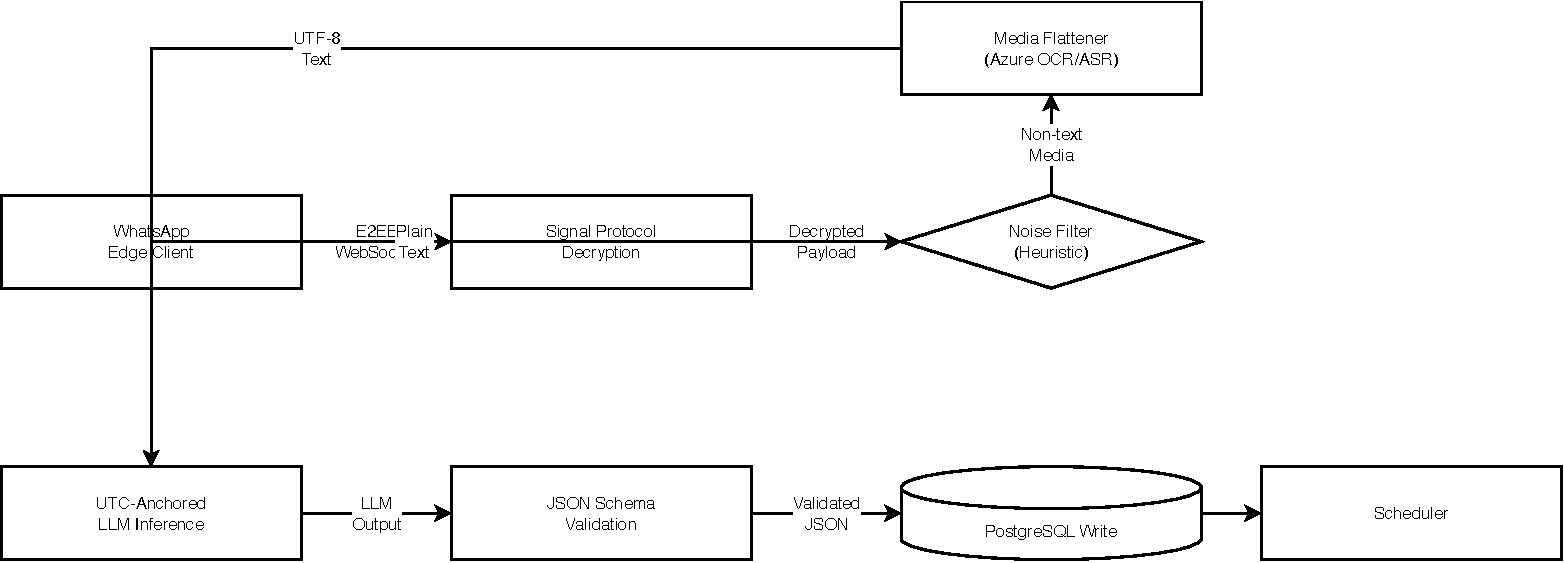
\includegraphics[width=0.90\textwidth,keepaspectratio]{figures/Fig3_Data_Flow_Diagram.pdf}
    \setlength{\abovecaptionskip}{4pt}
    \setlength{\belowcaptionskip}{-4pt}
    \caption{Data Flow Diagram showing the stateless information trajectory through the Chatnalyxer pipeline. E2EE payloads are decrypted at the edge, triaged, normalized, and destructively parsed. No intermediate state persists between the ingestion and storage stages.}
    \label{fig:dfd}
\end{figure*}

\subsection{UTC-Anchored Prompting Strategy}
Standard LLM inference has no access to the system clock. A message containing ``submit by tomorrow'' is semantically unambiguous to a human reader who knows today's date, but entirely unresolvable to a model that sees only the text. Without a temporal reference point, the model either hallucinates a plausible-sounding date or returns a null value—neither of which is acceptable in a scheduling application.

To resolve this, we prepend a machine-readable UTC anchor to every prompt before inference (Algorithm~\ref{alg:temporal_anchoring}). The anchor takes the form \texttt{[SYSTEM ANCHOR: CURRENT TIME IS 2026-07-07T14:30:00Z]}, derived from the message's network transmission timestamp. Given an explicit calendar position, the model can compute offsets for deictic expressions (``tomorrow'' $\rightarrow$ 2026-07-08, ``next Friday'' $\rightarrow$ 2026-07-12) and output valid ISO-8601 deadlines. Crucially, this requires no model fine-tuning—the grounding information is supplied entirely through the prompt context.

\subsection{Fallback Prompting and Output Validation}
LLMs are not designed to reliably produce valid JSON even when instructed to do so. Rare but real failure modes include truncated output, mismatched brackets, and schema field omissions. Rather than raising a pipeline error on the initial failure, Chatnalyxer implements a self-correction loop via \texttt{pydantic} schema validation. If validation fails, the malformed output and the Python exception traceback are re-injected into the LLM as a second prompt, asking the model to correct its own output against the schema. Only if this second attempt also fails does the pipeline raise a fatal error and discard the message. In practice, this two-attempt strategy recovers the vast majority of initially malformed responses.
